%marqueur aux points de données
% courbe en dessous/en dessus / intervalle dichotomie / condition d'arrêt / eps essai-erreur

Dans cette partie, nous résolvons le problème variationnel avec l'épaisseur fixée à $e=0.1$ m, à l'aide d'un programme FreeFem++.

% link free fem

\begin{problem}{3}
    Modélisons le pont, maillons-le et effectuons une simulation.
\end{problem}


\begin{solution}   
    En suivant les indications de l'énoncé, nous avons commencé par réaliser les bordures, correctement "orientées" et "subdivisées", de la coupe du pont (selon l'axe $y$),
    selon la méthode vue en cours sur les maillages.%faire varier n
    Nous avons ensuite maillé la surface à l'aide de la fonction \emph{buildmesh} de FreeFem++.
    On note $n$ le paramètre contrôlant le nombre de subdivisions pour une bordure du maillage.

    \begin{figure}      
        \begin{center}
        
            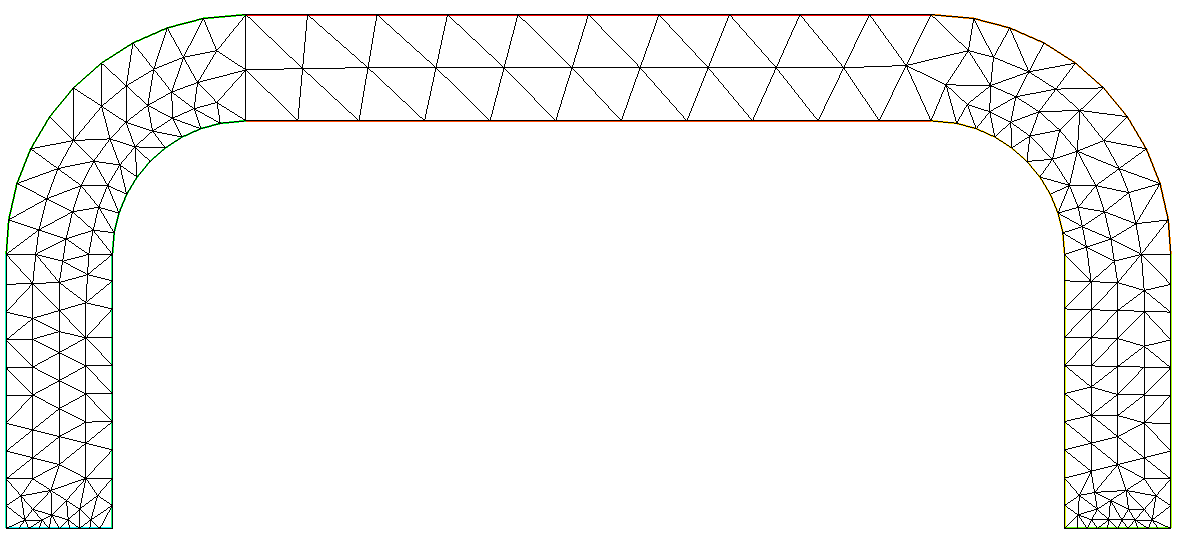
\includegraphics[width=12cm]{imgs/all_maillage_default.PNG}
            \caption{Maillage basique du pont}
            \label{fig:maillage_default}
        
        \end{center}
    \end{figure}

    On remarque cependant sur la figure \ref{fig:maillage_default} que la zone d'intérêt a un maillage très grossier, tandis que les pieds du pont sont très maillés. 
    On choisit donc de pondérer les subdivisions du maillage ($n/2$, $n$ et $2*n$), ce qui donne la figure \ref{fig:maillage_pondere}.
    
    \begin{figure}     
        \begin{center}
        
            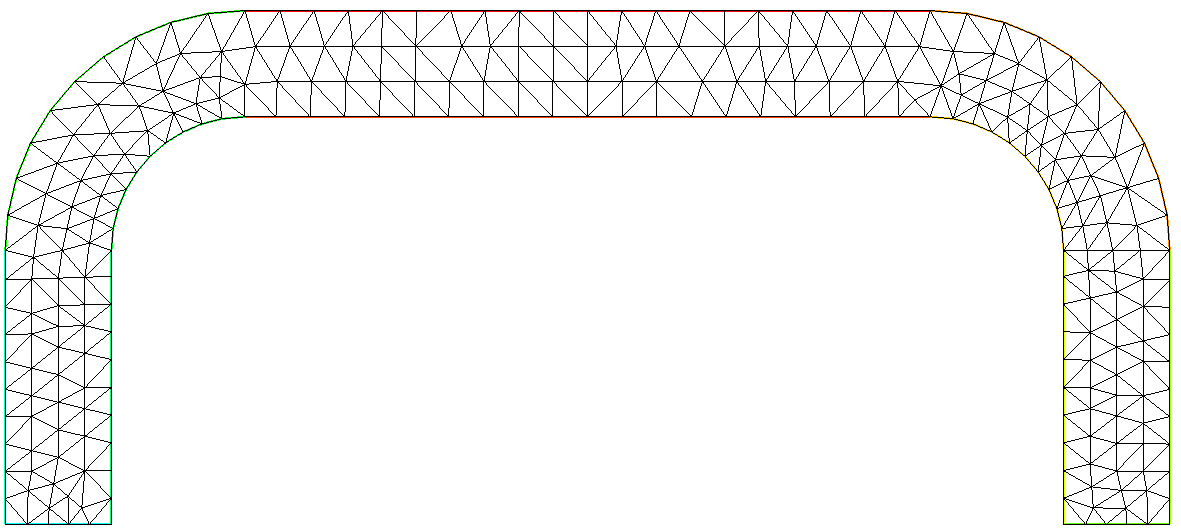
\includegraphics[width=12cm]{imgs/all_maillage_pondere.PNG}
            \caption{Maillage plutôt homogène du pont}
            \label{fig:maillage_pondere}
        
        \end{center}
    \end{figure}

    Ensuite, on donne de la profondeur afin de passer à un maillage 3D avec la fonction \emph{buildlayers} de FreeFem++, 
    avec un paramètre $m=n/2$ qui est le nombre de subdivisions de la bordure du maillage. On effectue après une rotation de la structure 
    avec la fonction \emph{movemesh3}, en pensant à spécifier \emph{orientation=-1} pour ne pas avoir un maillage non conforme.
    On obtient ainsi la figure \ref{fig:maillage_3d}.

    
    \begin{figure}        
        \begin{center}
        
            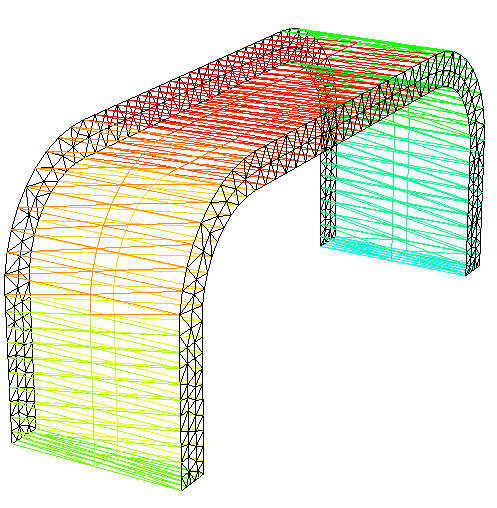
\includegraphics[width=6cm]{imgs/all_maillage_3d.PNG}
            \caption{Maillage 3D du pont}
            \label{fig:maillage_3d}
        
        \end{center}
    \end{figure}

    Après écriture de l'équation \ref{varia} dans le langage de FreeFem++, on obtient le déplacement en P en cherchant la déformation verticale minimum, ainsi que 
    l'aperçu de la structure déformée (Figure \ref{fig:simu_def}). 
    Sur les figures, $coef$ désigne le coefficient d'amplification du déplacement pour pouvoir l'observer, $dep$ le déplacement en P et $lateral$ 
    le déplacement maximal selon l'axe $y$ (tout est en mètres).
    
    \begin{figure}        
        \begin{center}
        
            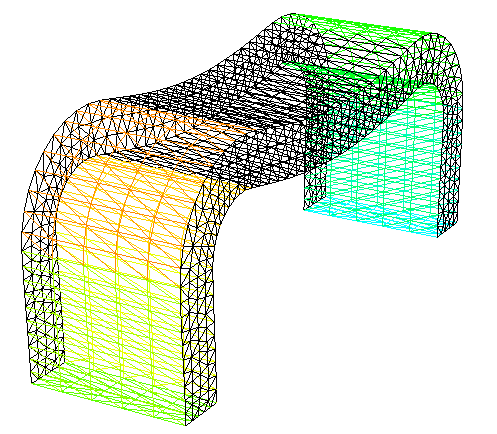
\includegraphics[width=6cm]{imgs/all_simu.PNG}
            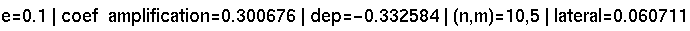
\includegraphics[width=12cm]{imgs/all_simu_label.PNG}
            \caption{Résultat d'une simulation de toute la structure}
            \label{fig:simu_def}
        
        \end{center}
    \end{figure}

    On peut réaliser la même démarche pour la moitié de la structure en utilisant l'équation \ref{moitie} (Figure \ref{fig:simu_def_moitie}).

    \begin{figure}        
        \begin{center}
        
            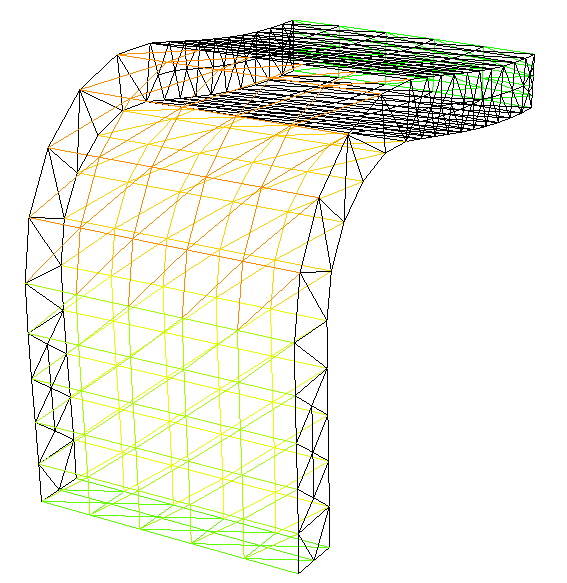
\includegraphics[width=6cm]{imgs/half_simu.PNG}
            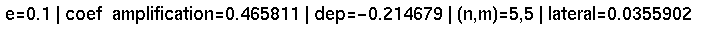
\includegraphics[width=12cm ]{imgs/half_simu_label.PNG}
            \caption{Résultat d'une simulation de la moitié de la structure}
            \label{fig:simu_def_moitie}
        
        \end{center}
    \end{figure}

\end{solution}

\begin{problem}{4}
    Retravaillons le maillage pour avoir de meilleurs résultats et vérifier les propriétés de convergence.
\end{problem}

\begin{solution}
    Nous avons implémenté une fonction d'adaptation du mesh automatique avec la fonction \emph{adaptmesh}

    Nous l'utilisons sur toute la structure et la moitié de la structure pour vérifier la cohérence.
\end{solution}
%critique : pas d'adapatation de m

%adapt mesh très mauvais maillage

% parallelization freefem

%optimisation temps

% étude convergence

% problème 2d équivalent
% adaptation de maillage 3d mmg3d et mshmet
% mumps, parallèle autre exécutable freefem
% erreur de valeur